%%%%% --------------------------------------------------------------------------------
%%
%%                               Document Template
%%
%%%%% --------------------------------------------------------------------------------
%% MODIFIED BY SEBASTIEN BLANCHET JULY 2017
%%%%% --------------------------------------------------------------------------------
%%
%%%%************************ Document Class Declaration ******************************
%%
\documentclass[singlesided]{Style/uwaterloothesis}% thesis template of University of Waterloo
%% Multiple optional arguments:
%% [<singlesided|doublesided|printcopy>] % single-sided, double-sided, or print layout
%% [draftversion] % show draft version information, default is no show
%% [standard options for book class]
%%%%% --------------------------------------------------------------------------------
%%
%%%%************************* Command Define and Settings ****************************
%%
\usepackage[list, table]{Style/commons}% common settings
%% Added packages
\usepackage{Style/custom}% user defined commands
%% For multi line equations
\usepackage{mathtools}
%\usepackage{amsmath}
%% For paragraph indentation, removes all indentation
\usepackage{parskip}
% for code import in appendix
\usepackage{listings}
% for proper figures placement
\usepackage{float}
% for properly formated section begining
\usepackage{titlesec}
\titleformat{\chapter}{\bf\normalfont\LARGE}{\bf\thechapter.}{20pt}{\LARGE\bf}
\titlespacing*{\chapter}{0pt}{0pt}{12pt}
\titlespacing*{\section}{0pt}{*1}{*1}
% for appendices
\usepackage[toc,page]{appendix}
% for pdf import
\usepackage{pdfpages}
% matrix
\usepackage{amsmath}

%%%%% --------------------------------------------------------------------------------
%%
%%%%******************************** Content *****************************************
%%
\begin{document}
%%
%%%%% --------------------------------------------------------------------------------



%%%%******************************** Frontmatter *************************************
%%
%% Frontmatter of Title page, Table of contents, Preface chapter.
\frontmatter
%%
%% >>> Frontpages
%%
%%
%% >>> Title Page
%%
%%\LaTeX{} is Latex printed in right way
%% Define new commands (add space after defined names0
\newcommand{\Term}{4A }
\newcommand{\Seb}{Sebastien Blanchet }
\newcommand{\DelivName}{Final Project: Combustor CFX Simulation}
\newcommand{\ReportTitle}{}
\newcommand{\Prof}{Cécile Devaud, PhD, PEng}
\newcommand{\CourseName}{ME 566: CFD for Engineering Design}

%% Define command variable names
\title[\DelivName]{\DelivName}% \title[short title for headers]{Long title of thesis}
\author{\Seb}
\preparedfor{\Prof}
\preparedcity{\CourseName}
\discipline{\Term Mechanical Engineering}
\maketitle

%%
%%% >>> List of Content
%%
%% Set TOC to record subsections
\setcounter{tocdepth}{3}
\setcounter{secnumdepth}{3}
%% TOC LOF LOT
\tableofcontents% contents catalog
\intotoc{\listfigurename}% add a corresponding item to the contents table and bookmark
\listoffigures% figures catalog
\intotoc{\listtablename}% add a corresponding item to the contents table and bookmark
\listoftables% tables catalog

%%%%% --------------------------------------------------------------------------------

%% >>> prematter
%%
%% input tex file
%%
% >>> Nomenclatures
%
\chapter{Glossary}
%% Symbols
\nomenclatureitem[\textbf{Unit (SI)}]{\textbf{Symbol}}{\textbf{Description}}
\nomenclatureitem[$\Unit{mm}$]{$a$}{Cylindrical Shell Radius}

%Greek
\nomenclatureitem[$\Unit{mm^{-1}}$]{$\beta$}{Thin Shell Parameter}
\nomenclatureitem[]{}{}

%% Acronym
\nomenclatureitem{\textbf{Acronym}}{\textbf{Description}}
\nomenclatureitem{ASME}{American Society of Mechanical Engineers}



%% >>> Summary
%%
\chapter{Summary}

The objective of this report is to perform a structural analysis on Altaeros' grounded TMS winch, focusing on the sizing of drum and flange thicknesses.\\

An external pressure $p=1376\Unit{psi}= 9.484\Unit{MPa}$ is calculated from the Capstan equation as a result of the tethers maximum tension. Initial drum thicknesses are determined by study of ASME's BPVC, EN, DNV and TWPV standards yielding a range of $t\in [0.825, 1.680]$ in / $\in [21.0, 43.2]$ mm.\\

The theory of thin shells is presented to setup analytical drum thickness results of 1.686 in / 42.8 mm. for a fixed end cylinder, loaded with uniform pressure $p$. Buckling analysis is also completed, resulting in 0.418 in / 10.6 mm for a critical buckling pressure of $p'=p$, confirming that buckling is not the primary mode of failure.\\

%%%%%
Utilizing various loading scenarios, FEA simulations are investigated. Run 1 yields 1.200 \& 0.875 in for uniform pressure $p$ and both fixed / simply supported ends, respectively. Run 2 yields 0.650 \& 0.550 for a Capstan pressure profile with fixed and simply supported ends, respectively. Run 3 yields a critical thickness of 0.375 in for a uniform critical buckling pressure $p'=p$ with simply supported ends. Run 4 yields 0.250 in as a preliminary flange thickness.\\

In summary, the drum barrel shall be manufactured with a Schedule 30 ($t=$ 0.625 in), 28 in OD pipe. Flanges should be cut from a $3\Unit{feet}^2$ by $0.250\Unit{in}$ thick plate.\\

Future works should focus on refining the flange design, nonlinear buckling, drum fatigue analysis as a result of changing tether loads and assembly proof testing.% list of symbols, preface of books
%%
%%%%%

%%%%******************************** Mainmatter **************************************
%%
%% Main topics.
\mainmatter
%%
%%% >>> Main Contents
%%
%%
%%% ++++++++++++++++++++++++++++++++++++++++++++++++++++++++++++++++++++++++++++++++++
%-----------------------------------------------------------------------------------------------------------------
\chapter{Introduction}
\label{ch:intro}


%-----------------------------------------------------------------------------------------------------------------
\chapter{CFX Pre}
\label{ch:pre}

\section{Reference}
\label{sec:pre_ref}


\section{Model 1}
\label{sec:pre_mod1}


\section{Model 2}
\label{sec:pre_mod2}


%-----------------------------------------------------------------------------------------------------------------
\chapter{Results \& Analysis}
\label{ch:res}

\section{Reference}
\label{sec:res_ref}


\section{Model 1}
\label{sec:res_mod1}


\section{Model 2}
\label{sec:res_mod2}


%-----------------------------------------------------------------------------------------------------------------
\chapter{Conclusions}
\label{ch:conc}

%%% ++++++++++++++++++++++++++++++++++++++++++++++++++++++++++++++++++++++++++++++++++


%%%%% --------------------------------------------------------------------------------
%%%%******************************* Backmatter ***************************************
%%
%% Matters of Bibliography, Glossary, Index.
\backmatter
%%
%%% >>> Bibliography
%%
%% Need to run bibtex in compiler 
\intotoc{\bibname}
%% Get IEEE reference style
\bibliographystyle{ieeetran}
\bibliography{Biblio/Refs}
%%

%%%%******************************** Appendix ****************************************
%%
\cleardoublepage
\backmatter
\chapter{Appendix A: CFX Results}
\label{appendix:cfx}
\hypertarget{appendixa}{}

\renewcommand{\thesection}{A.\arabic{section}}
\renewcommand\thefigure{A.\arabic{figure}} 

\section{Velocity $\vec{V}$}
\begin{figure}[H]
    	\centering
        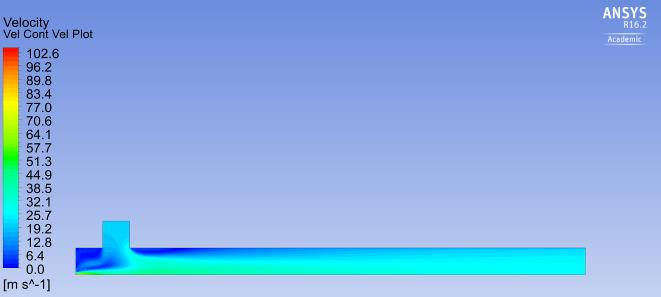
\includegraphics[width=\textwidth]{appendix/vel_ref}
        \caption{Reference velocity.}
        \label{fig:vel_ref}
\end{figure}
\begin{figure}[H]
    	\centering
        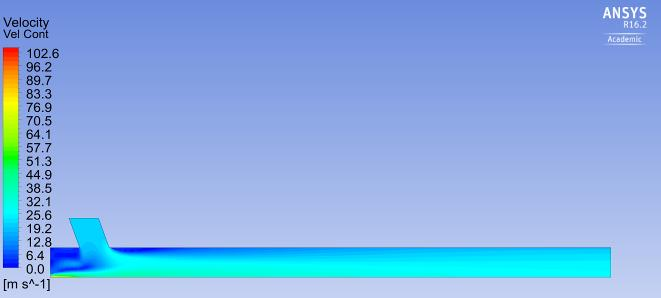
\includegraphics[width=\textwidth]{appendix/vel_mod1}
        \caption{Model 1 velocity.}
        \label{fig:vel_mod1}
\end{figure}
\begin{figure}[H]
    	\centering
        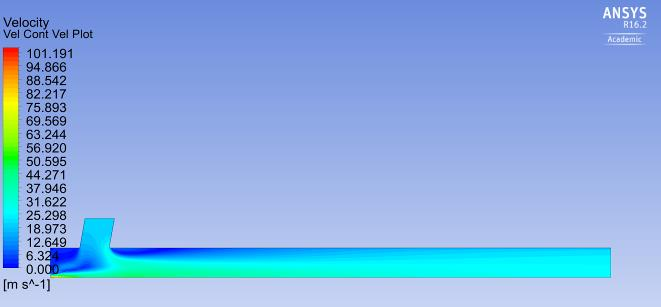
\includegraphics[width=\textwidth]{appendix/vel_mod2}
        \caption{Model 2 velocity.}
        \label{fig:vel_mod2}
\end{figure}

%------------------------------------------------------------------------------------------------------
\begin{figure}[H]
    	\centering
        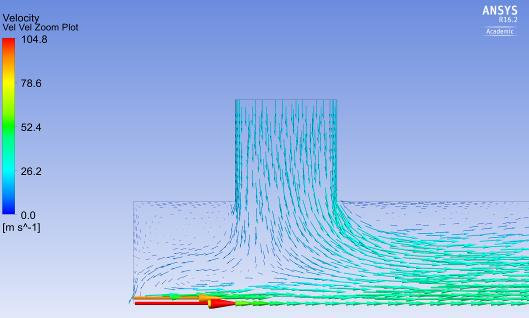
\includegraphics[width=\textwidth]{appendix/velz_ref}
        \caption{Reference velocity zoom.}
        \label{fig:velz_ref}
\end{figure}
\begin{figure}[H]
    	\centering
        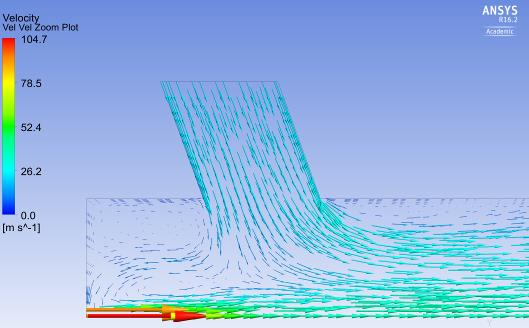
\includegraphics[width=\textwidth]{appendix/velz_mod1}
        \caption{Model 1 velocity zoom.}
        \label{fig:velz_mod1}
\end{figure}
\begin{figure}[H]
    	\centering
        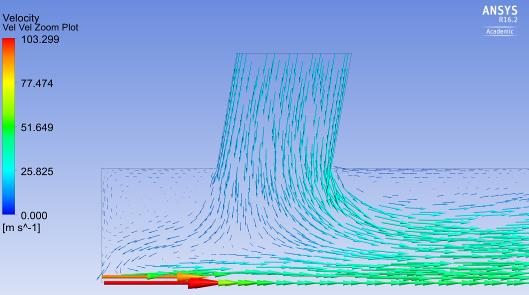
\includegraphics[width=\textwidth]{appendix/velz_mod2}
        \caption{Model 2 velocity zoom.}
        \label{fig:velz_mod2}
\end{figure}

%------------------------------------------------------------------------------------------------------
\section{Turbulent Kinetic Energy $k$}
\begin{figure}[H]
    	\centering
        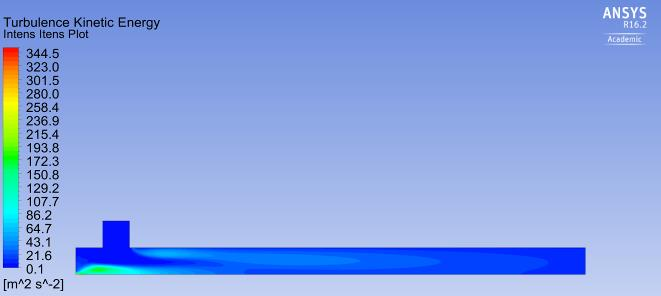
\includegraphics[width=\textwidth]{appendix/ke_ref}
        \caption{Reference turbulent kinetic energy.}
        \label{fig:ke_ref}
\end{figure}
\begin{figure}[H]
    	\centering
        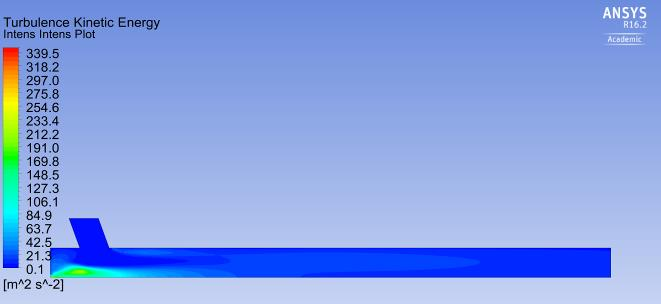
\includegraphics[width=\textwidth]{appendix/ke_mod1}
        \caption{Model 1 turbulent kinetic energy.}
        \label{fig:ke_mod1}
\end{figure}
\begin{figure}[H]
    	\centering
        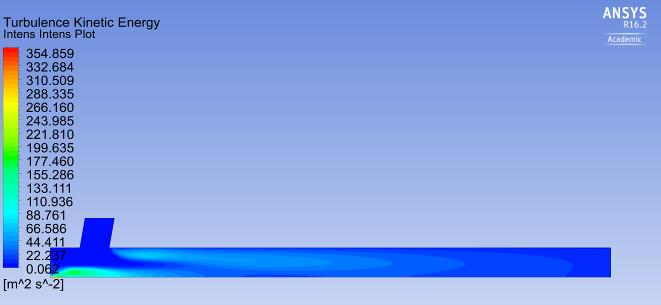
\includegraphics[width=\textwidth]{appendix/ke_mod2}
        \caption{Model 2 turbulent kinetic energy.}
        \label{fig:ke_mod2}
\end{figure}

%------------------------------------------------------------------------------------------------------
\section{Temperature $T$}
\begin{figure}[H]
    	\centering
        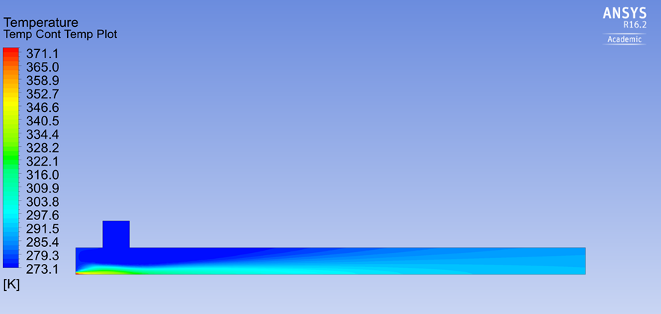
\includegraphics[width=\textwidth]{appendix/temp_ref}
        \caption{Reference temperature.}
        \label{fig:temp_ref}
\end{figure}
\begin{figure}[H]
    	\centering
        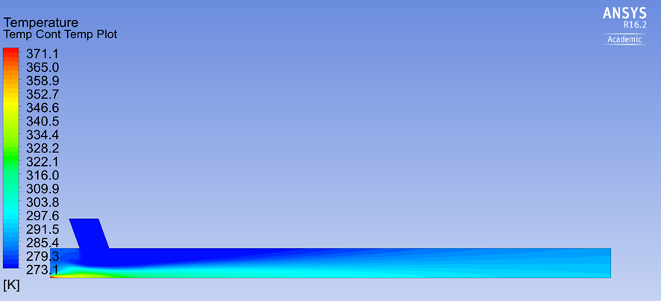
\includegraphics[width=\textwidth]{appendix/temp_mod1}
        \caption{Model 1 temperature.}
        \label{fig:temp_mod1}
\end{figure}
\begin{figure}[H]
    	\centering
        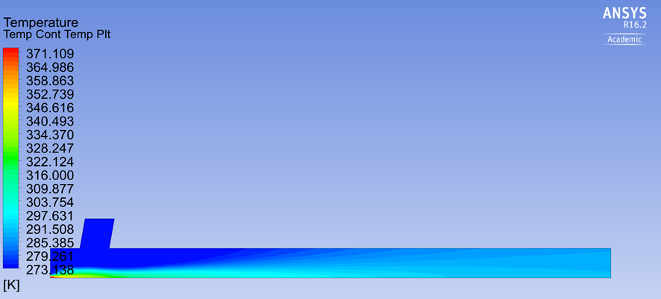
\includegraphics[width=\textwidth]{appendix/temp_mod2}
        \caption{Model 2 temperature.}
        \label{fig:temp_mod2}
\end{figure}


%------------------------------------------------------------------------------------------------------
\chapter{Appendix B: MATLAB Script}
\label{appendix:matlab}
\hypertarget{appendixb}{}
\nopagebreak
\begin{scriptsize}
	\lstinputlisting[language=MATLAB]{"C:/Users/Sebastien/Documents/GitHub/ME566/Project/MATLAB/data.m"}
\end{scriptsize}
%%%%%% --------------------------------------------------------------------------------

\end{document}
%%%%% --------------------------------------------------------------------------------
